\chapter{Estado del arte}\label{ch:estado-arte}

\section{Teoría de la evolución}

La computación evolutiva está basada, como muchos otros saberes humanos, en la
observación y funcionamiento de la naturaleza. Como la propia palabra anticipa,
la computación evolutiva imita al proceso de evolución natural para alcanzar
objetivos computacionales. Esta descripción es una breve explicación de ciertos
fenómenos naturales que nos servirán para entender mejor la computación
evolutiva.

¿Qué es el código genético?  El código genético es el conjunto de normas por las que la información codificada
en el material genético (secuencias de ADN o ARN) se traduce en proteínas (secuencias de aminoácidos) en las
células vivas. Esto significa que el código genético almacena toda la información física de nuestro cuerpo:
color de la piel, color de ojos, altura de las orejas, etc. No obstante, la información aprendida durante la
vida no se almacena en los genes (código genético). De esta forma, nuestros hijos se parecen a nosotros porque
llevan parte de nuestro código genético, sin embargo, no actúan de la misma manera, ya que el comportamiento
depende de muchos otros factores (educación, amistades, sociedad). Por ejemplo, los gemelos son idénticos
genéticamente y, por ello, su apariencia externa es la misma; pero su forma de actuar puede ser completamente
diferente.

El código genético está formado por una o varias cadenas de ácido
desoxirribonucleico o ADN. A su vez estas cadenas están formadas por cuatro
nucleótidos cuyas bases son: adenina (A), timina (T), citosina (C) o guanina (G).
Estas bases se unen entre sí formando largas cadenas de información
(AGGTACGTAATTCTGTCG…). Las secuencias de ADN que constituyen la unidad
fundamental, física y funcional de la herencia se denominan genes (figura
\ref{fig:adn}). De esta forma llamaremos gen a la parte de ADN que codifica, por
ejemplo, el color de los ojos. Realmente, toda esta información genética se asemeja a un lenguaje, y como todo
lenguaje, tiene reglas gramaticales y sintácticas, y una posterior interpretación
y expresión.

\begin{figure}[t] \centering
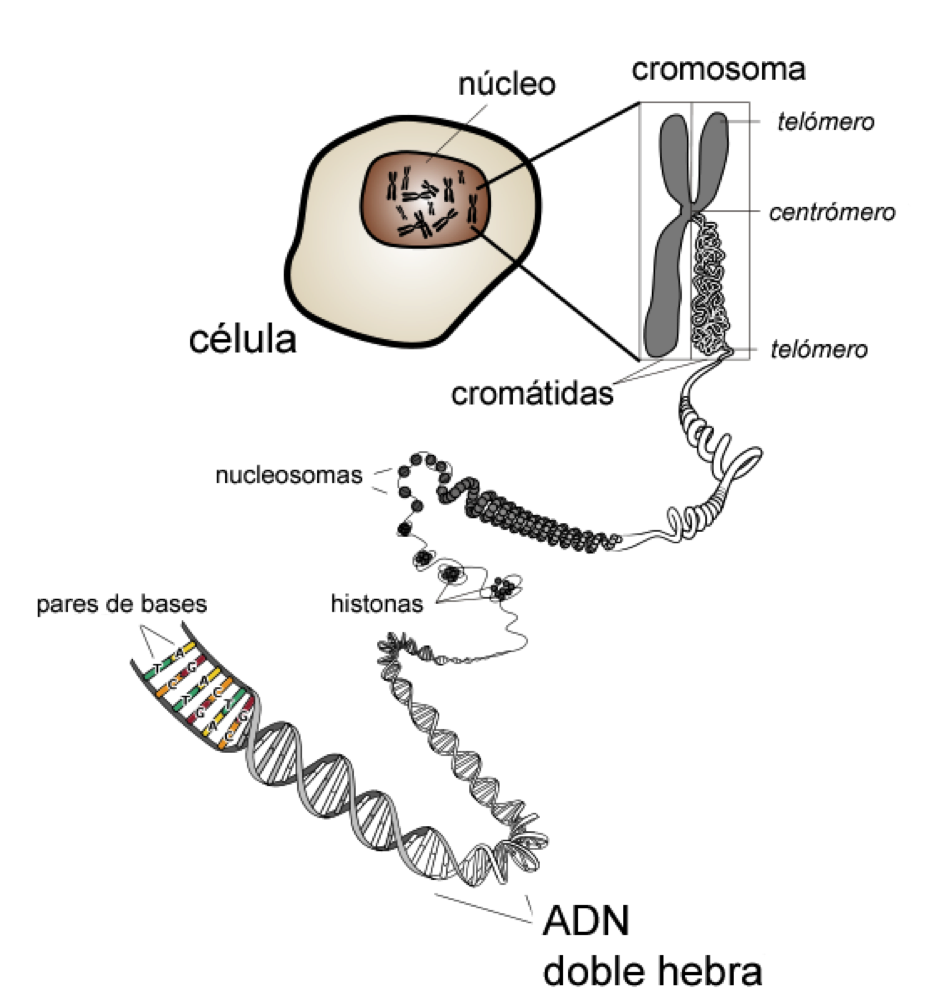
\includegraphics[width=0.45\textwidth]{figs/adn}
\caption{Estructura del ADN.}
\label{fig:adn}
\end{figure}

Sin embargo, existe una diferencia en la información que contiene el código
genético y la expresión del mismo. Eso es lo que llamamos genotipo y fenotipo. El
genotipo es la  información que nuestro código genético contiene. El fenotipo es
la expresión del genotipo. Ésta puede variar por diferentes motivos: dominancia
de genes, medio ambiente, etc. Por ejemplo: es posible tener información para los
ojos azules y marrones y poseer ojos marrones.

Cada individuo de una población tiene su propio ADN único que le define.  No
obstante, no dista mucho de otro individuo de su misma especie. De este modo
pueden reproducirse entre ellos. Esto se debe a que al tener trozos similares de
ADN, con la misma función, se pueden intercambiar por los mismos trozos del otro
individuo. Esto se llama cruzamiento. Así, la descendencia tendrá algunos rasgos
del padre y otros rasgos de la madre: su código genético se ha mezclado
(figura \ref{fig:mendel}).

\begin{figure}[t]
\centering
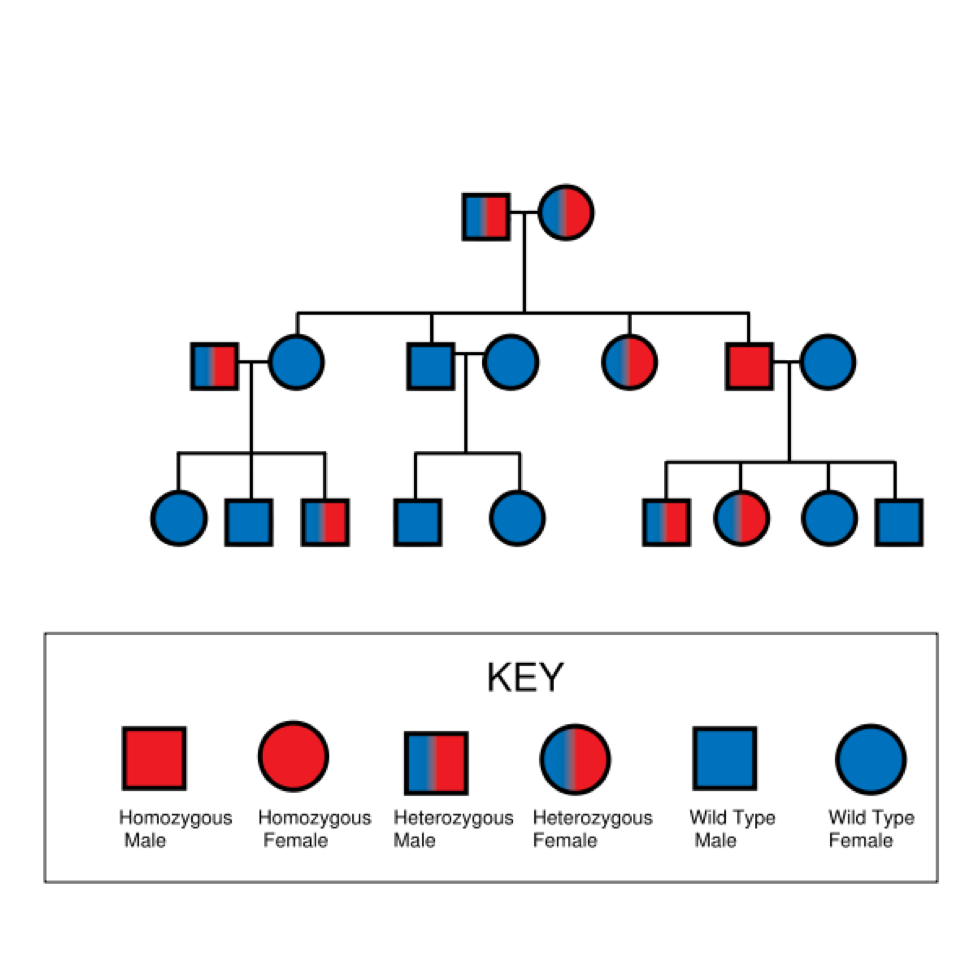
\includegraphics[width=0.45\textwidth]{figs/mendel}
\caption{Ejemplo de posibles descendencias y combinaciones de dos individuos con
dos tipo de gen (rojo y azul).}
\label{fig:mendel}
\end{figure}

Se ha demostrado que la diversidad es necesaria para la supervivencia de la
especie. Este hecho se hizo presente en la realeza Española a lo largo de la
historia, donde solo tenían descendencia entre ellos. La consanguinidad reducía
considerablemente la diversidad genética y empobrecía la calidad de lo
individuos, potenciando enfermedades genéticas. Por ejemplo, Carlos II nació
débil, estéril y enfermizo víctima de sucesivos matrimonios consanguíneos de la
familia real.

Por lo tanto, la naturaleza necesita ciertas similitudes para mezclar ADN, pero,
es fundamental que existan pequeñas diferencias en el ADN de los progenitores.
Esto es crucial para el éxito en la evolución: la diversidad.

La diversidad tiene su origen en la mutación. Una mutación es una alteración en
el código genético que produce cambios en el fenotipo. La consecuencia mas
importante de las mutaciones es que pueden ser heredadas por las siguientes
generaciones. No obstante, la mayoría de las mutaciones producen consecuencias
fatales para el individuo y sólo en contadas ocasiones tienen un resultado
positivo para la continuidad de la especie.  Por ejemplo una mutación que
cambie de color a un animal y por ello es capaz de camuflarse mejor con su
entorno.

La función de la diversidad es crear individuos capaces de ofrecer diferentes
desempeños en situaciones de diversa naturaleza. Estas situaciones pueden ser
fatales si no son superadas. Por ejemplo, el ataque de un determinado virus, o el
ataque de un depredador. Ciertas cualidades consiguen hacer que el individuo siga
viviendo y por lo tanto tener descendencia. Por lo tanto, podríamos decir que la
naturaleza selecciona a los individuos más aptos. Es lo que se llama selección
natural.

Combinando toda esta teoría evolutiva con la informática surge la computación
evolutiva.

\section{Computación evolutiva}

Desde que Von Neumann ideó su modelo de computación moderna en los albores de la
informática, el concepto de algoritmo tomó más fuerza que nunca (una secuencias
de pasos que sirve para resolver un problema). El problema ahora es encontrar la
secuencia de pasos adecuada. Con la ventaja de que estas “nuevas” máquinas eran
capaces de ejecutar estas secuencias de pasos infinitamente más rápido que el ser
humano, se abrió la puerta a nuevos campos de búsqueda y nuevas ideas. Desde
siempre la naturaleza ha aportado a nuestra civilización multitud de ideas y
soluciones y, en este ámbito, no iba a ser diferente. Por qué no imitar el
mecanismo que tiene la naturaleza para dar con sus excelentes soluciones. La
computación evolutiva es la implementación del algoritmo de la evolución.

Esta idea dio lugar a diferentes vertientes dentro de la computación evolutiva,
entonces inexistente como tal. Desde Estados Unidos, J. Fogel  \cite{Fogel:1966}
daba las primeras pinceladas a lo que se llamaría programación evolutiva. Fogel
creó un sistema evolutivo donde los individuos a evolucionar eran máquinas de
estado finito en el ámbito de la predicción. Henry Holland  \cite{Holland:1975}
tuvo otra visión de este concepto y quiso aplicarlo a problemas de optimización,
donde los individuos consistían en valores numéricos que se aplicaban de alguna
forma a un determinado algoritmo. Este método recibió el nombre de algoritmos
genéticos. En 1960 Ingo Rechenberg y Hans--Paul Schwefel  \cite{Rechenberg:1971}
propusieron las Estrategias Evolutivas. Sobre la base de los resultados previos,
Koza  \cite{Koza:1992} inició la última de las cuatro ramas, la programación
genética. En esta última, los individuos que evolucionan son programas informáticos que luchan por
conseguir la solución con mayor (o menor) puntuación.  El mejor programa será
capaz de procrear y tener descendencia, en cambio, los menos aptos estarán
predestinados a desaparecer.

En todas estas ramas es común tener una población de individuos que se reproducen
y/o mutan, permitiendo la descendencia a los individuos que consiguieron mejor
puntuación enfrentándose a un problema determinado. Sorprendentemente, el
algoritmo converge, tendiendo a que la población actual mejore la puntuación de sus
antecesores.

En computación evolutiva es necesario evaluar a cada individuo de la población y
para ello se necesita reproducir el entorno adecuado del problema que se quiere
resolver. Además, para asegurar el éxito de nuestro algoritmo, necesitamos un
gran número de individuos en la población. Esto hace que estos algoritmos
necesiten muchos recursos computacionales. Sin embargo, gracias a los últimos
avances tecnológicos, la computación evolutiva está en auge actualmente.

\section{Programación genética}

En 1992, John R. Koza publicó Genetic Programming: On the Programming of
Computers by Means of Natural Selection \cite{Koza:1992}, un libro que extiende y
asienta las bases que Nichael Lynn Cramer \cite{Cramer:1985} inició con su
publicación A Representation for the Adaptive Generation of Simple Sequential Programs.

Koza habla de las posibles codificaciones que un programa lineal puede tener
 para poder ser evolucionado. Defiende que la estructura más adecuada es la
representación en árbol. Un programa representado como árbol tiene múltiples
ventajas: Es posible volver al estado lineal sin ambigüedades. Las operaciones de
reproducción y mutación consumen menos recursos, además de producir mejor
rendimiento.

Este modelo de representación dio lugar a multitud de alternativas de
modificación y ajuste del algoritmo. Existen infinidad de posibilidades con los
que podemos “jugar” y probar, como los posibles métodos de reproducción,
mutación, inicialización de programas, selección de nodos, etc. Hablaremos de
estos aspectos en los siguientes apartados.

El algoritmo de la programación genética es como todos los algoritmos de la
computación evolutiva. Se trata de un bucle, donde cada iteración se llama
generación. En el caso de la primera iteración se creará una población de un
determinado número de programas aleatoriamente generados. Durante la iteración,
se procederá a la evaluación de los individuos, selección, reproducción,
mutación, y así sucesivamente.

En el proceso de evaluación, se ejecutará el programa y se puntuará de alguna
forma su comportamiento.

En el proceso de selección, se eligen los individuos más aptos de todas la
población para procrear y generar una nueva población. Para procrear se pueden
utilizar diferentes métodos, incluso puede darse el caso en el que los individuos
simplemente se clonen.
 
Una vez que tenemos la nueva población, se forzará la mutación de algunos
individuos con una cierta probabilidad.

El bucle de generaciones llegará a su fin cuando se encuentre al individuo ideal
(si es que puede llegar a existir un individuo que satisfaga todas nuestras
necesidades) o se llegue a un límite de generaciones.



\subsection{El problema del camino de la hormiga (Santa Fe Ant Trail)}

Antes de continuar, se describirá una aplicación de ejemplo muy característico en
la programación genética que servirá para la comprensión de los conceptos. Este
problema es el problema del camino de la hormiga o en inglés Santa Fe Trail Ant.
Consiste en conseguir que una hormiga situada en un mapa de rejilla pueda
seguir el ratro de comida. Este ratro de comida no es continuo. Así la hormiga
tendrá que seguir el ratro a pesar de las discontinuidades (ver figura \ref{fig:santa-fe}).

Evolucionar un individuo que resuelva este problema es un ejercicio de toma de
decisiones. Los individuos reciben información del ambiente; si hay o no comida
en frente de ellos y pueden moverse hacia adelante, girar a la izquierda o
girar a la derecha o una combinación de estos movimientos. El objetivo es comer
toda la comida posible en un periodo de tiempo determinado. Uno de los
motivos por el que se utiliza este problema para introducirnos a la
programación genética es que es sencillo y, sobre todo, mediante la programación
genética se puede resolver fácilmente este problema.


\begin{figure}[t] \centering
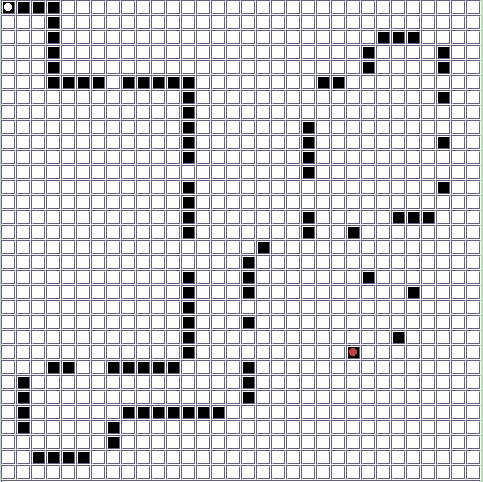
\includegraphics[width=0.65\textwidth]{figs/sftrail}
\caption{Representación del problema del camino de la hormiga de Santa Fe. Los
cuadrados negros representan comida, mientras que los cuadrados blancos están
vacío. El punto blanco es el punto de partida de la hormiga y el punto rojo es
el final del camino.}
\label{fig:santa-fe}
\end{figure}


\subsection{Lenguaje y árboles}

En la programación genética cada individuo tiene una determinada secuencia de
instrucciones a ejecutar, es decir, su propio código genético. Esta secuencia de
instrucciones es, como la propia palabra dice, secuencial. Por ello, muchas
implementaciones de sistemas de programación genética utilizan esta
representación para mezclar y evolucionar programas. Sin embargo, la
representación lineal dificulta las labores de reproducción ya que es difícil
encontrar zonas de similitud para intercambiar código. Asimismo, el intercambio
de código no asegura tener nuevos individuos sintácticamente correctos.

Existe otra forma de representación que aporta mayores alternativas a la hora de
crear y mezclar código genético: la representación en árbol. Es una de las más
extendidas en la programación genética debido a su flexibilidad y al gran número
de posibilidades que ofrece.

Un árbol es una estructura de datos formada por nodos. Un nodo, explicándolo de
una forma informal, es una caja que contiene dentro cierta información y que está
ligada a otras cajas, otros nodos. Estas ligaduras o conexiones se llaman hijos.
Existen nodos que podrán tener varios hijos, y nodos que no tendrán ninguno, en
cuyo caso se les llamará nodos hoja o terminales. Además existirá un nodo base
del que partirán el resto de los nodos (ver figura \ref{fig:arbol}).

\begin{figure}[t] \centering
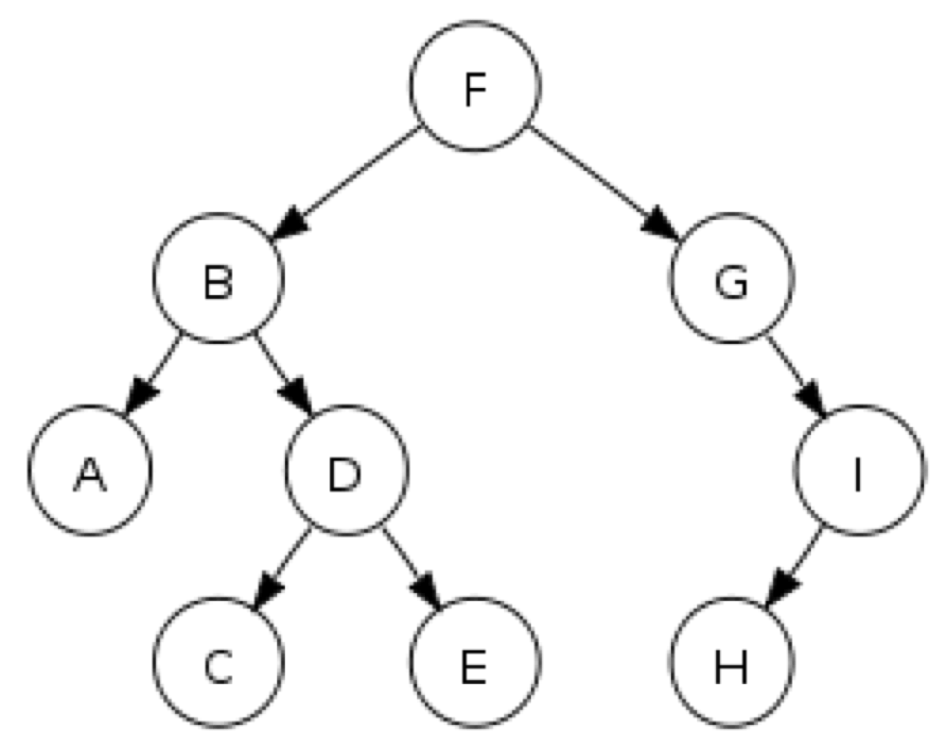
\includegraphics[width=0.45\textwidth]{figs/arbol}
\caption{Representación de un árbol.}
\label{fig:arbol}
\end{figure}

En la programación genética cada nodo contiene una instrucción del programa o una
constante. Las constantes suelen ser nodos terminales, y las instrucciones de
programa suelen ser nodos no-terminales.

Para ejecutar un programa, necesitamos una secuencia de instrucciones. Para
obtener una secuencia de instrucciones de un árbol existen una serie de
transformaciones que transforman estos árboles en un código lineal sin ningún
tipo de ambigüedad. Estas transformaciones se llaman preorder, inorder y
postorder:

Preorder: raíz, subárbol izquierdo, subárbol derecho. (F, B, A, D, C, E, G, I, H)
Inorder: subárbol izquierdo, raíz, subárbol derecho. (A, B, C, D, E, F, G, H, I)
Postorder: subárbol izquierdo, subárbol derecho, raíz. (A, C, E, D, B, H, I, G,
F)


La decisión de utilizar un orden especifico viene dado por el lenguaje que
apliquemos para resolver el problema.

Esta estructura es idónea para la reproducción de los programas, ya que facilita
el proceso de combinación genética que se representa por el intercambio de
subárboles y, en esta estructura, este proceso resulta trivial (cambiar un hijo
por otro).

En la ejemplo de la hormiga, el lenguaje serían todos los movimientos que puede
realizar la hormiga, además de la comprobación de si existe comida frente a ella.
Un pequeño árbol podría ser:

\begin{algorithmic}
\IF {$comidadelante$} 
    \STATE $avanzadefrente$
\ELSE 
	\STATE $avanzalateralmente$
\ENDIF 
\end{algorithmic}

\subsection{Etapas del proceso evolutivo}

El proceso evolutivo es un proceso iterativo, el cual se repite hasta que se
cumpla un criterio de parada. El criterio de parada puede ser que se haya llegado
a un máximo de iteraciones o que se haya encontrado al individuo deseado.

En la primera generación se inicializa la población, mediante procesos aleatorios
que debe proveer a la población de la suficiente diversidad para proporcionar el
éxito del algoritmo.

Después, el proceso iterativo se reduce a tres etapas: selección de individuos,
reproducción y adición de los nuevos individuos.

\subsubsection{Inicialización}\label{subsubsec:inittree}

La inicialización consiste en crear una nueva población y dotar a todos
los individuos de la población de un código genético admisible, además de generar
la diversidad suficiente en la población para que el sistema pueda evolucionar.
Se pueden llevar a cabo multitud de métodos para acometer este fin, sin embargo,
los más empleados y comunes son los métodos grow y  full que se suelen combinan
de forma que el 50\% de la población se genera por el método grow y el restante
con el método full. Estos métodos los describiremos a continuación.

El método grow genera un árbol de programa de un individuo aleatoriamente hasta
una determinada profundidad. En concreto, dado un conjunto de terminales  y de no
terminales de nuestro lenguaje, el método grow va rellenando el árbol
aleatoriamente escogiendo indiferentemente entre terminales y no terminales hasta
llegar a la máxima longitud, en cuyo caso sólo elije terminales terminando con la
expansión del árbol. Aunque existe un límite estipulado de longitud máxima, es
posible que los árboles generados no lleguen en profundidad a ese límite ya que
al escoger entre aleatoriamente entre símbolos terminales y no terminales, puede
darse el caso que aparezcan símbolos terminales podando el crecimiento del árbol.
Incluso es posible que los árboles generados tengan mayor longitud, ya que si
existe una gramática inherente al lenguaje, puede que en el límite de altura solo
podamos escoger símbolos no terminales, prolongando el crecimiento del árbol
hasta que podamos seleccionar terminales. Este método está muy condicionado por
la cantidad de nodos terminales y no terminales de nuestro lenguaje, ya que dado
un lenguaje con un alto número de terminales, la probabilidad de escoger uno
aumenta respeto a la probabilidad de escoger un símbolo no terminal. Esto ocurre
también al contrario.

El método full siempre escoge símbolos no-terminales hasta una determinada
profundidad donde, a partir de ahí, sólo elegirá símbolos terminales. Es por esto
que este método siempre genera árboles de la misma profundidad.
 
Como hemos mencionado antes, normalmente se utilizan ambos métodos para generar
la población inicial por el motivo de que el método grow está condicionado por el
número de terminales y no terminales del lenguaje, pudiéndose generar árboles muy
cortos en el caso que en el lenguaje predominen los símbolos terminales. Este
hecho puede poner en peligro el éxito de la evolución, ya que si los árboles que
generamos son demasiado cortos, la diversidad de la población no sería suficiente
para obtener la solución deseada. Sin embargo, el método full garantiza un mínimo
de altura en lo árboles, pero generando siempre árboles de la misma forma. Es por
esto por lo que se combinan ambos métodos, produciendo un número determinado de
individuos con un método y el resto con el otro.

Por último resaltar que en un lenguaje donde predominen los símbolos
no-terminales, los árboles generados con el método grow serán parecidos a los que
genere el método full.

\subsubsection{Evaluación}

Antes de proceder a la selección, es necesario evaluar a la población. El
proceso de evaluación consiste en ejecutar cada individuo y probar su eficacia
al solucionar el problema. Esa eficacia tendrá que ser codificada para poder
comparar a dos individuos cualquiera y decidir cuál es el mejor de ambos.

Para tomar esta decisión, podemos dar a cada individuo una calificación
numérica de su rendimiento. Una vez que tenemos esta calificación, la toma de
decisiones se simplifica al comparar que programa supera en calificación al otro
programa en cuestión. Además, tenemos que tener en cuenta si queremos maximizar
esta calificación, en cuyo caso, 0 sería el valor del individuo menos apto, e
infinito el individuo más apto; o si queremos minimizarla, en cuyo caso 0
representaría el individuo ideal e infinito el individuo menos apto.  Koza se
inclina a utilizar la segunda versión de calificación. A esta forma de puntuación
se la llamó fitness estandarizado. Además existe una transformación que acota
esta calificación entre 0 y 1, donde 0 sería el individuo peor y 1 el mejor. Esta
última calificación ajustada se la llamó a fitness ajustado. La transformación se
realiza mediante la siguiente formula:
\begin{equation}
   Adj = \frac{1}{1+f},
\end{equation} donde $f$ es el fitness estandarizado.


No obstante, en determinadas ocasiones, es difícil obtener una única nota por individuo, puesto que es posible
que existan diferentes medidas que influyen en la decisión.  Estos problemas surgieron sobretodo cuando se
detectó la aparición de bloat. El bloat son las partes del código del un
programa que carecen de sentido o son innecesarios. Para evitar este fenómeno se quiso introducir una medida más de control del bloat en la toma de decisiones de los individuos. Para combinar estos dos objetivos, se pensó utilizar una combinación lineal de los objetivos del tipo
\begin{equation}
   fitness = \sum_{i}w_if_i(x),
\end{equation}
donde $f_i(x)$ es el valor obtenido al evaluar la $i$-ésima función objetivo y  $w_i$ el valor por el cual
misma se poderará.

Incluso se puede llegar a tener una ponderación exponencial de los objetivos, cuando queremos dar mucha mas
importancia a un objetivo que a otro. Es posible, además, impedir el uso de un determinado objetivo hasta un
cierto nivel de satisfacción de otro objetivo.

Sin embargo, hay que prestar especial atención a la hora de combinar todos nuestros objetivos ya que es posible
que limitemos la evolución de nuestros programas si elegimos unos parámetros incorrectos. Por ello conviene
realizar un estudio previo del rendimiento de nuestro fitness.

Langdon y Poli \cite{LangdonPoli:1998} utilizaron un función semilineal para
combinar el acierto del programa y la velocidad para mejorar el rendimiento de la programación genética en el problema de la hormiga. No obstante, necesitaron
ajustar este fitness para aquellas hormigas que eran muy rápidas pero no conseguían resolver el problema.

Pero la combinación lineal de objetivos no es la única aproximación posible para resolver problemas
multi-objetivo, existen otros métodos capaces de optimizar varios objetivos simultáneamente, por ejemplo,
métodos basados en la optimización de la frontera de Pareto.

La frontera de Pareto es aquella frontera formada por las soluciones óptimas de una población. Estas soluciones
no se pueden comparar ya que, si por ejemplo observamos la figura
\ref{fig:pareto}, en algún punto una solución A ofrece mejor resultado frente a cierto problema que una solución B, sin embargo la B ofrece mejor solución a otro problema que la A. Por ello no se pueden comparar.
Sin embargo puede existir una solución C cuyas soluciones sean peor que la dada por la A, en ese caso, A es
estrictamente superior que C. Este sistema intenta evitar que la solución se quede en un mínimo local, ampliando
las fronteras a otros mínimos de interés. Además tiene la ventaja de potenciar la diversidad.

\begin{figure}[t]
\centering
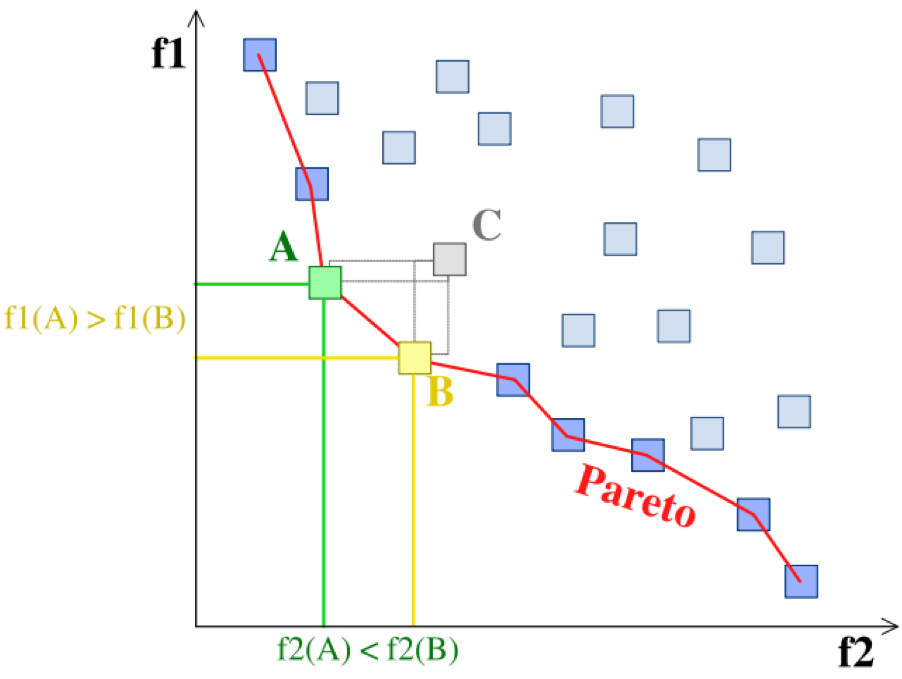
\includegraphics[width=0.65\textwidth]{figs/pareto}
\caption{Ejemplo de la frontera de Pareto.}
\label{fig:pareto}
\end{figure}

Además de la frontera de Pareto, existen otros métodos como el orden lexicográfico (los objetivos son ordenados
según la preferencia del usuario),  métodos basados en prioridades, otros métodos basados en la dominancia de la
frontera de Pareto pero con la adhesión de la cuenta del número de objetivos que un individuo es mejor que otro.
Incluso, es posible combinar varios métodos de evaluación, para conseguir una visión más objetiva y diversa
del problema. 

\subsubsection{Selección}

El proceso de selección sirve para escoger a los individuos de la población mejor
adaptados, para que actúen de progenitores de la siguiente generación. En la
naturaleza existen varios factores que intervienen para que un individuo pueda
tener descendencia. El primero de todos es que consiga sobrevivir, ya sea por que no es
devorado por depredadores, o porque sea capaz de procurarse alimento. Lo segundo
es que encuentre pareja para reproducirse. El último factor es que la
combinación de ambos individuos sea apta para crear un nuevo individuo. Sin
embargo, en la realidad es posible que “el mejor” individuo no pueda
reproducirse, pero otro individuo de “peor calidad” pueda conseguirlo. Aunque
este hecho es menos probable, sigue siendo posible.

En la programación genética, la selección es un conjunto de reglas que sirven para elegir a los progenitores de
la siguiente generación. Estos progenitores se reproducirán (cruzamiento genético) y generarán descendencia.

Un sistema muy utilizado en programación genética es la selección por torneo (tournament selection).  Este
sistema consiste en escoger aleatoriamente de la población un cierto número de individuos. De esos individuos se
escoge el mejor de todos para ser el padre. Para escoger la madre se repite el proceso: se escoge aleatoriamente
a un número de individuos de la población y se elige al individuo con mejor calidad. Este sistema garantiza un
mínimo de diversidad, ya que no siempre se elegirá al mejor individuo de la población para tener descendencia y
por lo tanto, no todos los hijos tendrán al mismo padre. Pero, por el contrario, existen grandes posibilidades
de que éste tenga descendencia, ya que si es escogido en algún torneo, será el vencedor.

Además existen otros métodos que no solo tienen en cuenta si un individuo es mejor que otro, sino que miden
también la diferencia de la calidad, ya que si la diferencia no es muy grande, quizás el vencedor de la
selección no es el que tenga un desempeño estrictamente superior.


\subsubsection{Reproducción}

La fase de reproducción es la que se encarga de generar nuevos individuos,
preferiblemente diferentes, a partir de los predecesores seleccionados en el
proceso anterior. En esta fase se pueden utilizar varios métodos de reproducción.
El cruzamientos es un método que consiste en intercambiar parte del código del
padre y parte del de la madre. Otro método más simple es el de la clonación, cuya
función consiste en copiar a los progenitores en la nueva población. Además, para
generar más variedad, los individuos son mutados con cierta probabilidad, esto es
que el código genético de algunos individuos es modificado introduciendo nuevo
material genético dentro de la población (figura \ref{fig:cross}).

\begin{figure}[t]
\centering
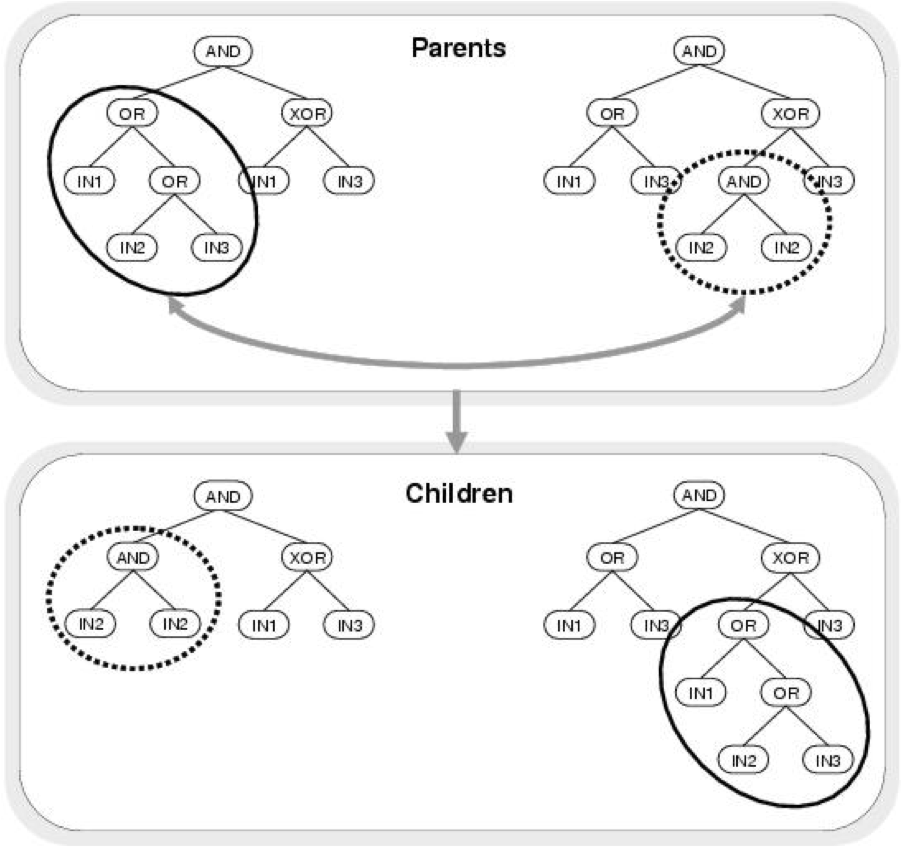
\includegraphics[width=0.55\textwidth]{figs/cross}
\caption{Cruzamiento de dos árboles.}
\label{fig:cross}
\end{figure}

Dependiendo del problema, nos interesará utilizar cruzamiento o clonación y mutación, o una combinación de estos
operadores controlados por probabilidades de aparición.
 
\paragraph{Cruzamiento}\label{para:crossover}

El cruzamiento es el intercambio de material genético entre dos individuos para producir un individuo nuevo y
diferente. En programación genética esto se traduce en intercambio de subárboles. Cuando dos individuos se van a
reproducir se selecciona un nodo aleatoriamente en el padre y otro nodo en la madre y se realiza el intercambio
de subárboles.

Sin embargo, en la naturaleza, durante la reproducción sexual de dos individuos se intercambia parte del código
genético de tal forma que el nuevo código genético generado es similar al de los padres. Esto es posible debido
a la organización existente del código genético en genes y cromosomas. En la programación genética  no sucede
exactamente de la misma forma ya que resulta muy costoso identificar las partes de código similares entre dos
programas. Es por ello que el código genético se almacena en árboles, imitando los genes y cromosomas en la
naturaleza. De esta forma se consigue estructurar el código genético de tal forma que puedan encontrarse partes
similares fácilmente. No obstante, la simple estructuración del código genético del programa en árboles no es
suficiente y requiere de subprogramas adicionales que controlen la reproducción ya que el intercambio de
subárboles sin control mismo puede cambiar radicalmente la configuración del árbol resultante, produciendo
efectos fatales.

Existen varios métodos denominados métodos homólogos que intentan preservar la
posición del material genético. Mantener la posición física del material
genético es trivial cuando se trata de programas lineales ya que en su forma
natural ya son lineales. Sin embargo, este proceso resulta más tedioso cuando
el código se encuentra almacenado en árboles ya que la transformación a código
lineal puede verse afectada enormemente por un ligero cambio en el arbol.

El más viejo operador de cruzamiento homólogo en programación genética es el
cruzamiento en un punto. El operador intercambia un subárbol que coincida en la
raíz en los dos padres. Identifica las partes con la misma forma estructural
(misma aridad\footnote{En el análisis matemático, se define a la aridad de un
operador matemático o de una función como el número de argumentos necesarios para
que dicho operador o función se pueda calcular.}), e intercambia el código
genético a partir de estas partes comunes. De esta forma, este sistema intenta
mantener la posición original del código genético intercambiado
\cite{LangdonPoli:2002}.

El método de cruzamiento de tamaño similar escoge el primer nodo de forma aleatoria como el cruzamiento normal.
Sin embargo, el segundo nodo debe seleccionarse de tal forma que la altura de este segundo subárbol debe ser
parecida a la altura del primer subárbol seleccionado.
 
Harries y Smith \cite{HarriesSmith:1997} idearon cinco operadores nuevos de
cruzamiento muy parecidos a los tradicionales pero con restricciones de profundidad en los puntos de cruzamiento de los árboles de los padres utilizando un criterio
probabilístico.

No obstante, existen otras clases de operadores lineales de cruzamiento, pero pertenecen a una representación
distinta a la utilizada, por lo que no nos concierne para el desarrollo del proyecto. 

\subparagraph{Clonación}

Como su propio nombre dice, se trata de copiar individuos de una generación a otra. Este método se llama también
reproducción, aunque en este contexto el nombre puede dar lugar a ambigüedades. Clonar no aporta nueva
diversidad a la población, no obstante, en ciertas ocasiones resulta conveniente aplicarlo, sobre todo en las
ocasiones donde se ha conseguido una solución muy óptima y no se desea perder la información correspondiente a
esa solución.

Al ser un operador que pone en peligro la diversidad de la población se suele utilizar con probabilidades muy
bajas o nulas. Por otro lado, es cierto que en la naturaleza existen especies que utilizan la clonación como
forma de reproducción, pero siempre se da en organismos sencillos. Por otro lado, existen estudios que
demuestran que posible evolucionar individuos con clonación combinada con mutación.

Por otro lado existe un sistema de los algoritmos evolutivos llamado elitismo que es un mecanismo para preservar
a los individuos más aptos de la población clonando a estos individuos en la nueva población.


\subparagraph{Mutación}

En el ámbito de la programación genética la mutación se define como el cambio aleatorio del código genético
(código de programa) del individuo. Este cambio se puede producir en cualquier punto del código y actuar de las
siguientes formas: borrando código, generando código o cambiando una instrucción por otra.

La mutación, al producirse de forma aleatoria, produce efectos incontrolados y genera individuos menos aptos
para la supervivencia. Por ello, la frecuencia de aparición de este fenómeno suele ser baja. Incluso se ha
llegado a cuestionar si es necesario para que el algoritmo evolutivo converja. Se ha demostrado que es posible
resolver problemas con programación evolutiva sin llegar a utilizar la mutación. Sin embargo, la mutación debe
entenderse como un punto de entrada de diversidad. Y si no somos capaces de generar esa diversidad en el inicio
del algoritmo, la mutación salvará a la población de quedarse estancada.

A diferencia de los programas lineales donde una mutación solo produce un cambio puntual en el material
genético, las mutaciones en los árboles pueden aparecer de diversas formas, que se explican a continuación:

 \begin{enumerate}
    \item La mutación de subárbol selecciona un nodo aleatoriamente y genera un
    subárbol aleatorio para ese nodo \cite{Koza:1992}.
    Kinnear \cite{Kinnear:1993} amplió este método restringiendo la profundidad
    del árbol producido a un 15\%.

	\item La mutación de reemplazo de nodo selecciona un nodo al azar y lo
	reemplaza por un nodo equivalente, de la misma aridad y mismas propiedades. Este método se parece a la versión lineal de reemplazar una línea de código
por otra.

	\item La mutación Hoist genera un nuevo individuo a partir de un subárbol del
individuo anterior. La raíz del nuevo árbol será diferente al del anterior y el árbol generado será más pequeño.

	\item La mutación Shrink intercambia un subárbol elegido aleatoriamente por un
nodo terminal aleatorio compatible. Este método también reduce el tamaño final del programa.


	\item La mutación de permutación selecciona un nodo aleatoriamente e
intercambia de posición sus subárboles. Es posible que en algunos casos, este intercambio no refleje ningún cambio en el funcionamiento del programa.

\end{enumerate}

\subsubsection{La nueva población}

Una vez que hemos seleccionado, reproducido y con cierta probabilidad mutado la
población, es el momento de generar otra población con nuevos individuos.
Normalmente se escogen los nuevos individuos más aptos y se rellena la población
hasta un número máximo de individuos. Además, se puede reservar un espacio de
esta población para los individuos más aptos, con mejor puntuación, de la
generación anterior. Esto se llama elitismo. Aunque el elitismo apueste en contra
de  la diversidad, se ha comprobado que en ciertas ocasiones acelera la
convergencia del algoritmo, sin embargo, debe utilizarse con precaución. Además
al crear esta nueva población podemos encontrar dos formas de hacerlo: El modo
generacional y el modo de estado estacionario.

En el modo de estado generacional el sistema almacena todas las generaciones en espacios diferentes. Los nuevos
individuos ocupan un nuevo espacio. Este modo evolutivo aporta un gran valor
estadístico e incluso sería posible que antiguos individuos interviniesen en
nuevas poblaciones ya que poseemos la información de todos los
individuos de la evolución. El único inconveniente de este sistema es que requiere muchos más recursos y puede
ser un modo poco factible para largas ejecuciones.

En el modo de estado estacionario, el espacio asignado para almacenar los
programas siempre es el mismo, de esta forma, los nuevos individuos tienen que
desplazar a los individuos antiguos, ocupando su posición. Este método resulta
ideal para ejecuciones muy largas, poblaciones muy extensas o individuos que
ocupen mucho espacio en memoria. Incluso, es posible que en determinadas
ocasiones, el sistema ofrezca un rendimiento más alto que el sistema
generacional, ya que no tiene que generar nuevas estructuras, ni preocuparse por
clonar los individuos antiguos para crear nuevos. Lo único que tiene que hacer es
mantenerlos en la población.

\subsection{El cubo de Rubik}

El cubo de Rubik fue inventado por un profesor de arquitectura Húngaro Ernö Rubik
en 1974. Se trata de un puzzle en forma de cubo de 6 caras y con 9 pegatinas
coloreadas en cada cara.  Cada cara tiene un color y estas caras se pueden rotar
descolocando las posiciones de los colores. El objetivo del juego es volver a
juntar las pegatinas del mismo color.

La dificultad del cubo de Rubik radica en las millones de posiciones diferentes
que puede llegar a tener. En total se calcula que pueden existir más de 43
millones de permutaciones \cite{wiki:Rubik}.

Existen diversas formas de resolución del cubo de Rubik, no obstante, el misterio está en que no es posible
formalizar un algoritmo capaz de encontrar una solución óptima (la que menos pasos requiere) de cualquier cubo
desordenado. En 2008, Tomas Rokicki  \cite{Rokicki:2008} estableció el record
mas reciente y demostró que cualquier cubo de Rubik se resuelve en 22 movimientos o menos.

Estos algoritmos se basan en la búsqueda de todo el espacio de posibilidades del cubo de Rubik, el cual, es tan
grande que se puede tardar varias décadas en calcular. Para simplificar ligeramente el proceso se utiliza la
descomposición matemática del cubo de rubik en subconjuntos. Estos subconjuntos son más fáciles de resolver y
ofrecen una guía para estos algoritmos.

En nuestro sistema solo vamos a poder realizar movimientos de caras. Por lo tanto ya que tenemos 6 caras y dos
sentidos de movimientos, podremos hacer 12 movimientos en cada estado. Si tenemos un cubo ordenado, podremos
hacer 12 desplazamientos. Estos 12 cubos diremos que pertenecen a la dificultad 1. Por cada uno de estos 12
cubos tendremos 12 movimientos, por lo tanto 144 posibilidades. Estos cubos pertenecerán al nivel 2. Nótese que
12 de estos 144 cubos, es el cubo resuelto. Del nivel 3 tendremos 1.728 cubos y así en adelante.

Estos niveles de dificultad nos servirán para clasificar los cubos de Rubiks y tener una noción a priori del
número de pasos que son requeridos para su resolución.

Para referirnos a las caras del cubo utilizaremos la nomenclatura desarrollada
por David Singmaster  \cite{Singmaster:1981}:

\begin{itemize}
  \item F(Front): la cara que de enfrente. 
  \item B(Back): la cara opuesta a la frontal. 
  \item U(Up): la cara de encima a la frontal. 
  \item D(Down): la cara de debajo de la frontal.
  \item L(Left): la cara a la izquierda de la frontal. 
  \item R(Right): la cara a la derecha de la frontal.
\end{itemize}

Esta nomenclatura estandariza el caso de los posibles movimientos del cubo y hace posible expresar una posible
solución de forma rigurosa y sin ambigüedades.